\documentclass[spanish,11pt,letterpaper]{article}

\usepackage[spanish]{babel}
\usepackage[utf8]{inputenc}
\usepackage{authblk}
\usepackage{amsmath}
\usepackage{amssymb}
\usepackage{amsthm}
\usepackage[margin=1in]{geometry}
\usepackage{graphicx}
\usepackage{hyperref}
% \usepackage{listings}
% \usepackage{xcolor}

\renewcommand{\vec}[1]{\mathbf{#1}}
\DeclareMathOperator*{\argmax}{arg\,max}
\decimalpoint

\title{{\Huge Is this Loss?}\\
Sistema de reconocimiento de objetos en imágenes}
\author{Hernández Chiapa David Felipe\\
López García Gilberto Isaac}
\affil{Facultad de Ciencias\\Universidad Nacional Autónoma de México}
\date{\small\today}

\begin{document}

\maketitle

\section{Introducción}

\section{Descripción del problema}

\section{Redes Neuronales Convolucionales}

\subsection{Capa de convolución}

\subsection{Pooling}

\subsection{Perceptrón Multicapa}

\subsection{Espacio de Hipótesis}

\subsection{Ventajas y desventajas}

\section{Propuesta e implementación}

\subsection{Datos}

El conjunto de datos consiste de una colección de 1735 imágenes (1304 para
entrenamiento y 431 para verificación), divididos en
dos categorías, \texttt{loss\_edits} y \texttt{not\_loss}, donde la primera son
edits de Loss, y la segunda memes variados.

Los memes variados se obtuvieron de la colección personal de memes de los
desarrolladores, obtenidas con el paso del tiempo ya sea descargándolas de
distintos sitios de internet como redes sociales, chats de WhatsApp, Messenger,
etc., mientras que los edits de Loss se descargaron principalmente de la galería
de \textsf{KnowYourMeme.com}\footnote{\url{http://knowyourmeme.com/memes/loss/photos}} y
\textsf{Google Images} (que son miniaturas de distintos sitios, como el subreddit
\textsf{r/lossedits}\footnote{\url{http://reddit.com/r/lossedits}} y
\textsf{KnowYourMeme.com} por lo que puede haber imágenes repetidas en el dataset).

\subsubsection{Preprocesamiento}

El primer paso fue cambiar la resolución de las imágenes para tener un dataset
más uniforme (aunque se reescalarán posteriormente de nuevo pues la red neuronal
necesita entradas de tamaño fijo). Dado que las miniaturas de edits tienen baja
resolución (entre 200 y 300 pixeles de ancho/alto), los memes variados fueron
reescalados para tener una resolución similar (250 pixeles de ancho), después se
dividió el conjunto completo de imágenes en conjuntos de entrenamiento y
verificación de manera aleatoria.

Algunos edits de Loss se basan en el uso de colores, pero en general es la
orientación de los polígonos lo que importa como se ve en la Figura ~\ref{fig:im1}.
Para tratar estos casos se construyen modelos que trabajan con imágenes a color
y modelos que trabajan con imágenes en escala de grises.

\begin{figure}[h]
\centering
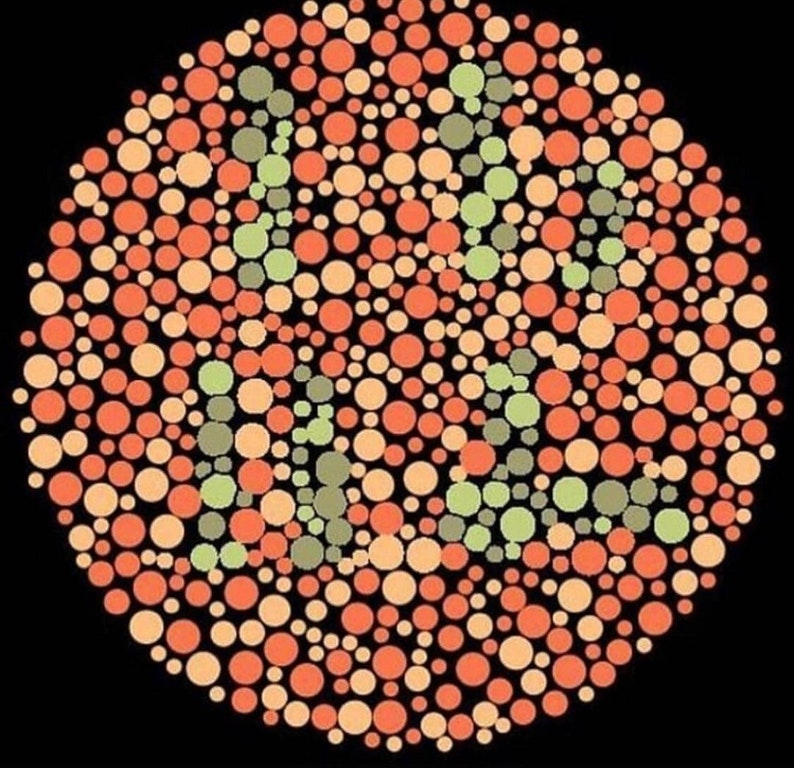
\includegraphics[height=3cm,width=3cm]{loss_color}
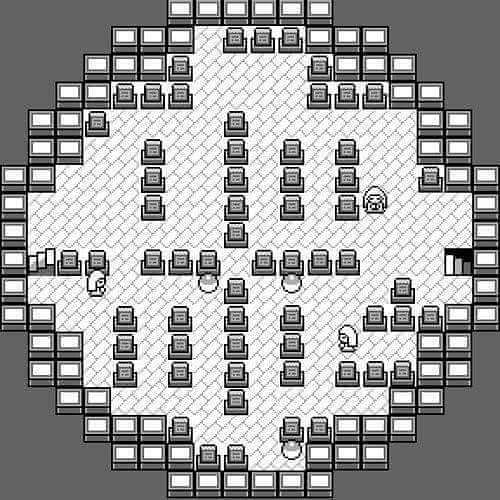
\includegraphics[height=3cm,width=3cm]{pokemon}
\caption{Edit basado en color (izq.) y en orientación (der.)}
\label{fig:im1}
\end{figure}

Procesar las imágenes para obtener las aristas se consideró una propuesta poco
viable pues se tiene mucho ruido o se pierde información. Usando el modelo
\textsc{Canny} de \textsc{OpenCV} para obtener las aristas presentes en una imagen
nos encontramos con mucho ruido, por ejemplo, si un edit se contruyó con fotografías
con muchos detalles en ellas y objetos innecesarios no fueron desenfocados, las
aristas de dichos objetos se extraen en conjunto con los polígonos que nos
interesan. Si modificamos los umbrales inferior y superior del modelo para filtrar
aristas podemos eliminar aristas de los objetos que nos interesan realmente. Estos
problemas se pueden apreciar en la Figura ~\ref{fig:im2}

\begin{figure}[h]
\centering
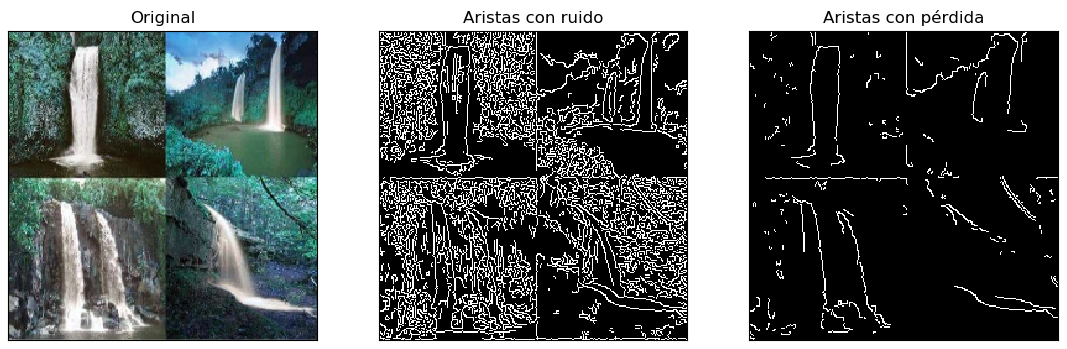
\includegraphics[width=0.9\textwidth]{edges}
\caption{Detección de aristas, algoritmo de Canny.}
\label{fig:im2}
\end{figure}

Además, los umbrales inferior y superior pueden no funcionar en distintas imágenes,
entregrando mucho ruido o pérdida de información. La baja resolución de las imágenes
también dificulta este proceso.

\subsection{Implementación}

La implementación se realizó en el lenguaje de programación \textsc{Python}%
\footnote{Versión 3.6.4, \url{http://www.python.org/downloads/release/python-364/}}.
Para la construcción de la red neuronal convolucional nos apoyamos de los
paquetes \textsc{TensorFlow}\footnote{\url{http://www.tensorflow.org/}} y
\textsc{Keras}\footnote{\url{http://keras.io}}.

\section{Resultados}

\subsection{Pruebas preliminares}

\subsection{Primer intento de clasificación}

\subsection{Segundo intento de clasificación}

\subsection{Observaciones}

\section{Conclusiones}

\begin{thebibliography}{9}
\bibitem{haykin}
Haykin, S. S. (2011).
\textit{Neural networks and learning machines}.
New Dehli: PHI Learning.

\bibitem{wuj}
Wu, J. (2018).
\textit{Convolutional neural networks}.
National Key Lab for Novel Software Technology. Nanjing University, China.
Obtenido de \url{http://cs.nju.edu.cn/wujx/teaching/15_CNN.pdf}.

\bibitem{pooling}
Scherer, D., M\"uller, A., \& Behnke, S. (2010).
\textit{Evaluation of Pooling Operations in Convolutional Architectures for Object Recognition}.
Artificial Neural Networks-ICANN 2010 Lecture Notes in Computer Science, 92-101. DOI:10.1007/978-3-642-15825-4\_10.

\bibitem{adagrad}
Ducji, J., Hazan, E., \& Singer, Y. (2011).
\textit{Adaptive Subgradient Methods for Online Learning and Stochastic Optimization}.
Journal of Machine Learning Research 12, 2121-2159.

\bibitem{adam}
Kingma, D. P. \& Lei Ba, J. (2014).
\textit{Adam: A Method for Stochastic Optimization}.
arXiv:1412.6980. Obtenido de \url{http://arxiv.org/pdf/1412.6980.pdf}.

\end{thebibliography}

\end{document}
